\documentclass[a4paper, 11pt]{article}
\usepackage[utf8]{inputenc}
\usepackage[english]{babel}
\usepackage[utf8]{inputenc}
\usepackage[margin=2.cm]{geometry}
\usepackage{fancyhdr}

\usepackage[T1]{fontenc}
\usepackage{lmodern}

\usepackage{graphicx}
\graphicspath{ {images/} }
\usepackage{pdflscape}


\usepackage{array}

\usepackage{multirow}

\usepackage{color,array}

\definecolor{mygray}{gray}{0.6} %custom color for text

\usepackage{float}
\usepackage[table,xcdraw]{xcolor}


\usepackage{varwidth} %for lists next to each other

%for subfigure
\usepackage{subcaption}


%Includes "References" in the table of contents
\usepackage[nottoc]{tocbibind}

\usepackage{enumitem}
\setlist{nolistsep}

\fancypagestyle{plain}{%
  \renewcommand{\headrulewidth}{0pt}%
  \fancyhf{}%
  \fancyfoot[L]{\footnotesize Raymond Lochner}
  \fancyfoot[C]{\footnotesize November 2017 - Université libre de Bruxelles}%
  \fancyfoot[R]{\thepage}
}
\pagestyle{plain}

\date{\today}

\begin{document}

\begin{titlepage}
	\centering
	{\scshape\LARGE Université libre de Bruxelles \par}
	\vspace{1cm}
	{\scshape\Large INFO-F-409 - Learning Dynamics\par}
	\vspace{1.5cm}
	{\huge\bfseries {Assignment Two\par}}
	\vspace{0.5cm}
	{\Large Evolutionary dynamics in a spatial context\par}
	\vspace{2cm}
	{\Large Raymond Lochner - 000443637\par}
	\vspace{0.5cm}
	{\Large raymond.lochner@ulb.ac.be}
	\vfill
	
	\setcounter{tocdepth}{2} %hides subsubsections in TOC
	\tableofcontents

\vfill
% Bottom of the page
	{\large \today \par}
\end{titlepage}

\newpage

\section*{Preliminary information}

Each game configuration was being simulated 100 times to receive a good picture of the various possible outcomes. Rounds were played until convergence was certain. For the visualizations:
\begin{itemize}[noitemsep]
  \item Red signifies the action \textit{cooperation}
  \item Blue signifies the action \textit{defection}
\end{itemize}

The graphic displays one specific game, whereas the cooperation graph shows information of all games combined.


\begin{figure}[H]
	\centering
    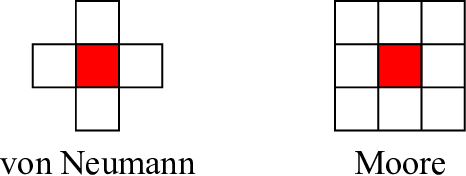
\includegraphics[width=0.9\linewidth]{NeighborhoodType}
    \caption{Two Neighborhood types}
\end{figure}


The tested games are:
\begin{itemize}[noitemsep]
  \item Weak Prisonners Dilemma - (T=10, R=7, P=S=0)
  \item Snowdrift Game - (T=12, R=7, P= 0, S=3)
\end{itemize}

\newpage
\section{Part One - Spatial Prisoners Dilemma}
\subsection{Moore Neighborhood}


%%%% 4x4
%%%%%%%%%%%%%%%%%%%%%%%%%%%%%%%%%%%%%%%%%
\subsubsection{4x4}
\begin{figure}[H]
\centering
\begin{subfigure}{.16\textwidth}
  \centering
  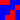
\includegraphics[width=0.9\linewidth]{PRISONERS_DILEMMA_MOORE_4x4_t00}
  \caption{t=0}
\end{subfigure}%
\begin{subfigure}{.16\textwidth}
  \centering
  
\includegraphics[width=0.9\linewidth]{PRISONERS_DILEMMA_MOORE_4x4_t01}
  \caption{t=1}
\end{subfigure}%
\begin{subfigure}{.16\textwidth}
  \centering
  
\includegraphics[width=0.9\linewidth]{PRISONERS_DILEMMA_MOORE_4x4_t05}
  \caption{t=5}
\end{subfigure}%
\begin{subfigure}{.16\textwidth}
  \centering
  
\includegraphics[width=0.9\linewidth]{PRISONERS_DILEMMA_MOORE_4x4_t10}
  \caption{t=10}
\end{subfigure}%
\begin{subfigure}{.16\textwidth}
  \centering
  
\includegraphics[width=0.9\linewidth]{PRISONERS_DILEMMA_MOORE_4x4_t20}
  \caption{t=20}
\end{subfigure}%
\begin{subfigure}{.16\textwidth}
  \centering
  
\includegraphics[width=0.9\linewidth]{PRISONERS_DILEMMA_MOORE_4x4_t50}
  \caption{t=50}
\end{subfigure}
\caption{Prisoners Dilemma, Moore, 4x4}
\end{figure}

\begin{figure}[H]
\begin{subfigure}{.75\textwidth}
	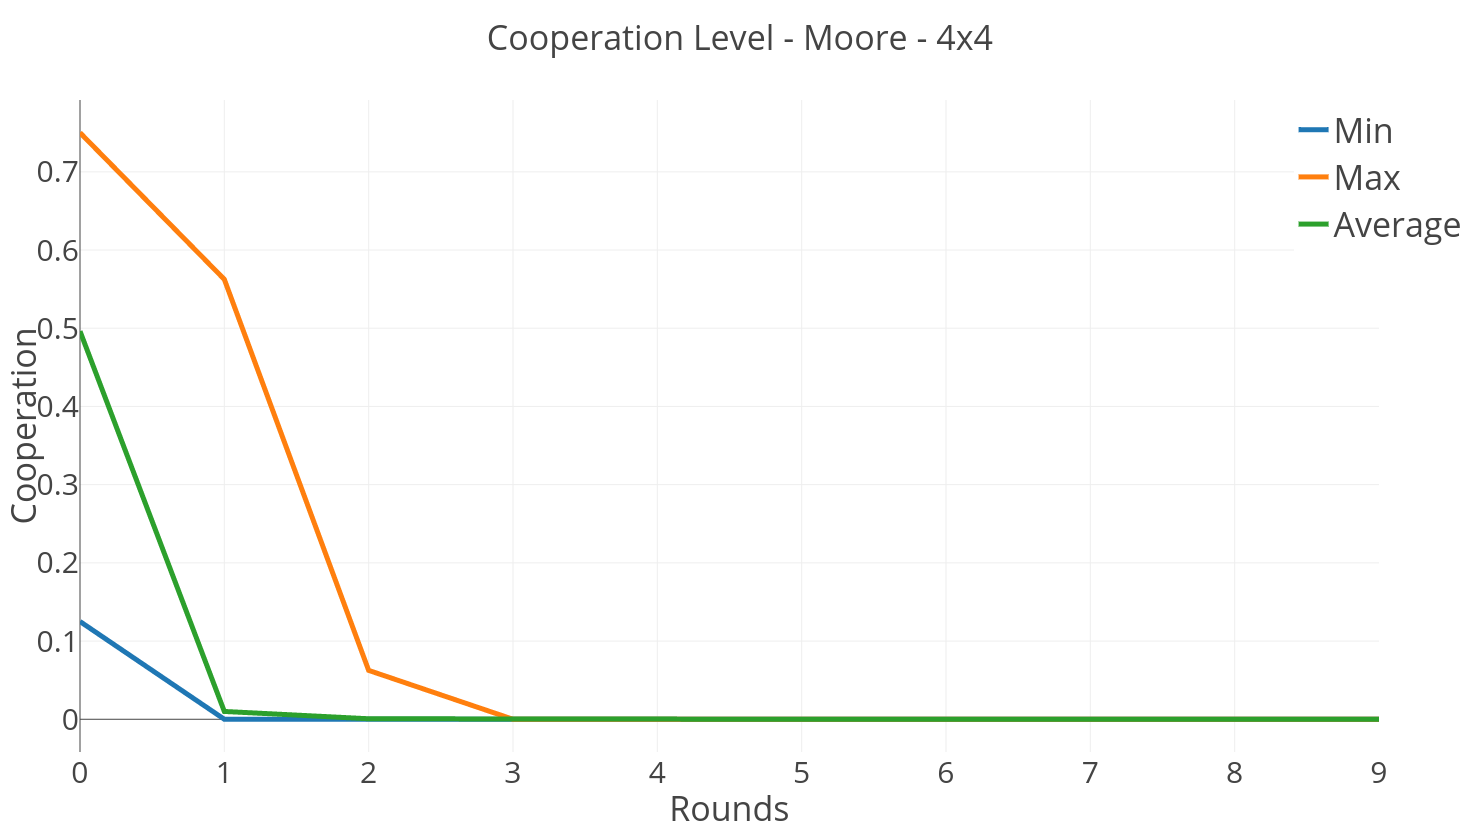
\includegraphics[width=1\linewidth]{PDMoore4x4}
\end{subfigure}

\begin{subfigure}{.75\textwidth}
	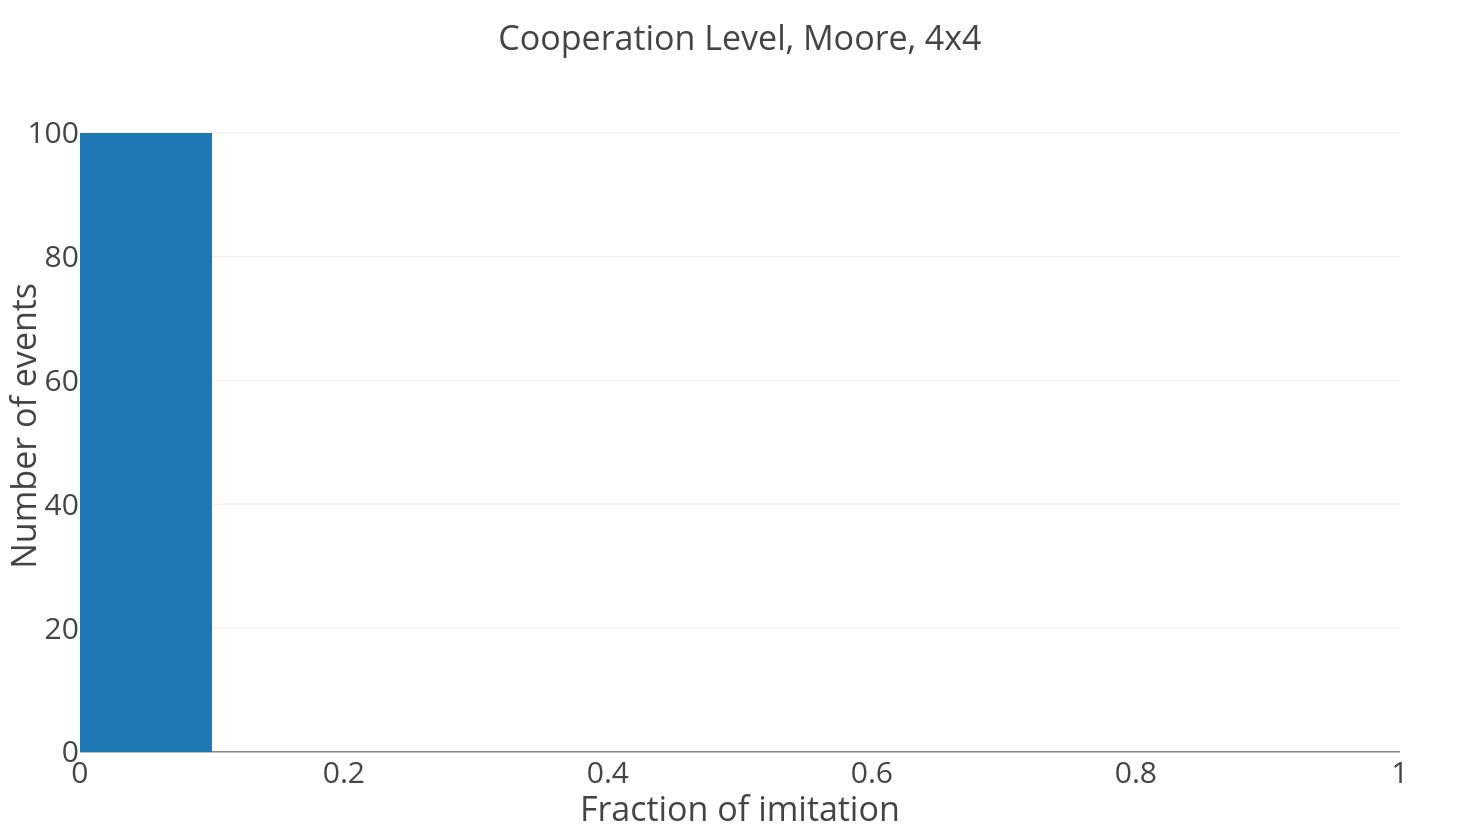
\includegraphics[width=1\linewidth]{PDMoore4x4HG}
\end{subfigure}%
\begin{subfigure}{.25\textwidth}
	mean = $0$
	
	deviation = $0$
\end{subfigure}

\end{figure}

	From simulating 100 runs we observe that all converge to the pure strategy of \textit{defecting} after 3 rounds. Nevertheless, it is however possible that a 4x4 configuration converges to a total cooperative field, but it requires that we have a sub-matrix of 2x2 with only cooperators and all other players being defectors. This did obviously not happen during one of the simulations.


\newpage

%%%% 8x8
%%%%%%%%%%%%%%%%%%%%%%%%%%%%%%%%%%%%%%%%%
\subsubsection{8x8}
\begin{figure}[H]
\centering
\begin{subfigure}{.16\textwidth}
  \centering
  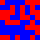
\includegraphics[width=0.9\linewidth]{PRISONERS_DILEMMA_MOORE_8x8_t00}
  \caption{t=0}
\end{subfigure}%
\begin{subfigure}{.16\textwidth}
  \centering
  
\includegraphics[width=0.9\linewidth]{PRISONERS_DILEMMA_MOORE_8x8_t01}
  \caption{t=1}
\end{subfigure}%
\begin{subfigure}{.16\textwidth}
  \centering
  
\includegraphics[width=0.9\linewidth]{PRISONERS_DILEMMA_MOORE_8x8_t05}
  \caption{t=5}
\end{subfigure}%
\begin{subfigure}{.16\textwidth}
  \centering
  
\includegraphics[width=0.9\linewidth]{PRISONERS_DILEMMA_MOORE_8x8_t10}
  \caption{t=10}
\end{subfigure}%
\begin{subfigure}{.16\textwidth}
  \centering
  
\includegraphics[width=0.9\linewidth]{PRISONERS_DILEMMA_MOORE_8x8_t20}
  \caption{t=20}
\end{subfigure}%
\begin{subfigure}{.16\textwidth}
  \centering
  
\includegraphics[width=0.9\linewidth]{PRISONERS_DILEMMA_MOORE_8x8_t50}
  \caption{t=50}
\end{subfigure}
\caption{Prisoners Dilemma, Moore, 8x8}
\end{figure}


\begin{figure}[H]
\begin{subfigure}{.75\textwidth}
	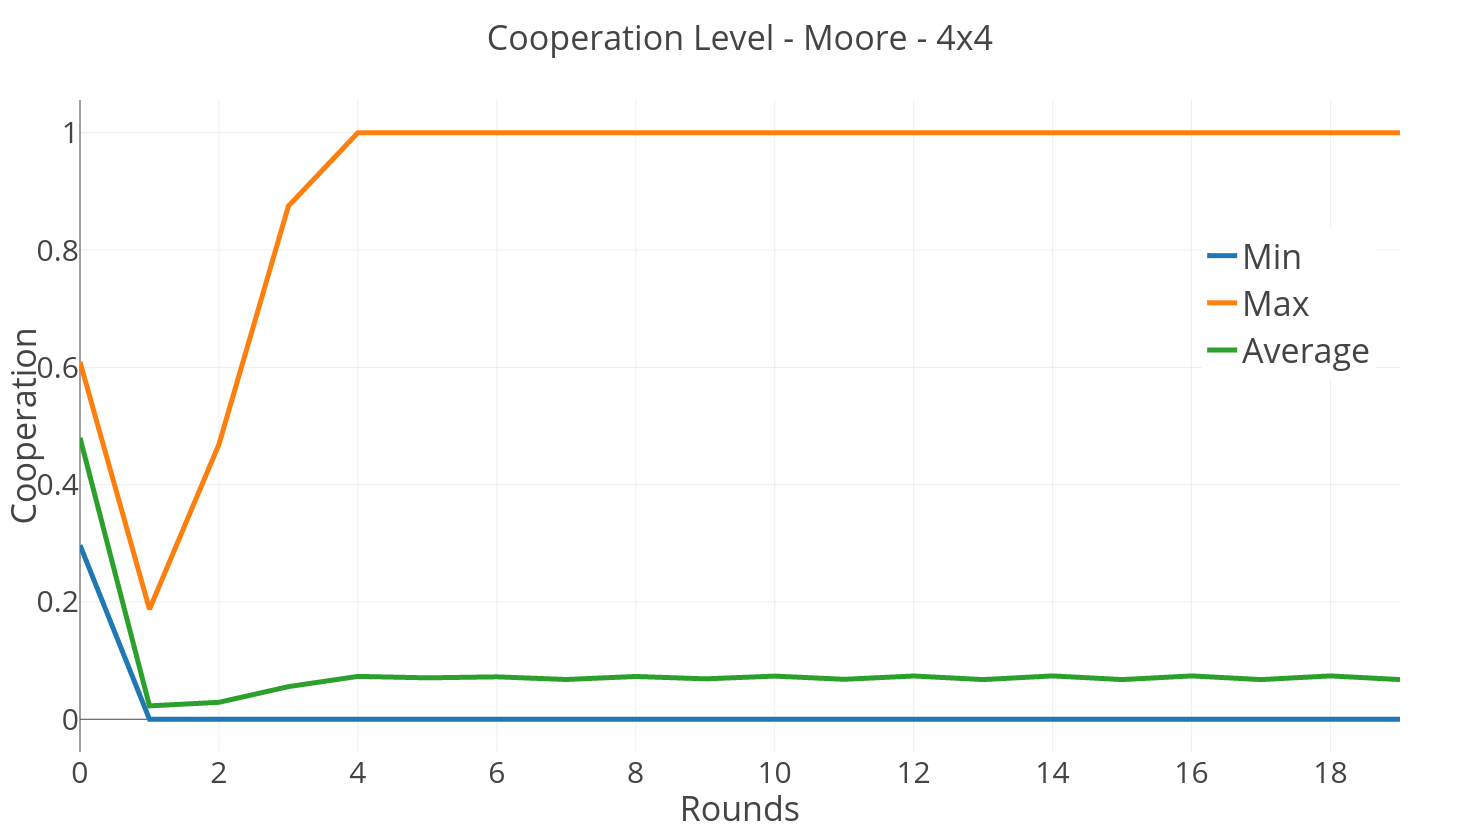
\includegraphics[width=1\linewidth]{PDMoore8x8}
\end{subfigure}

\begin{subfigure}{.75\textwidth}
	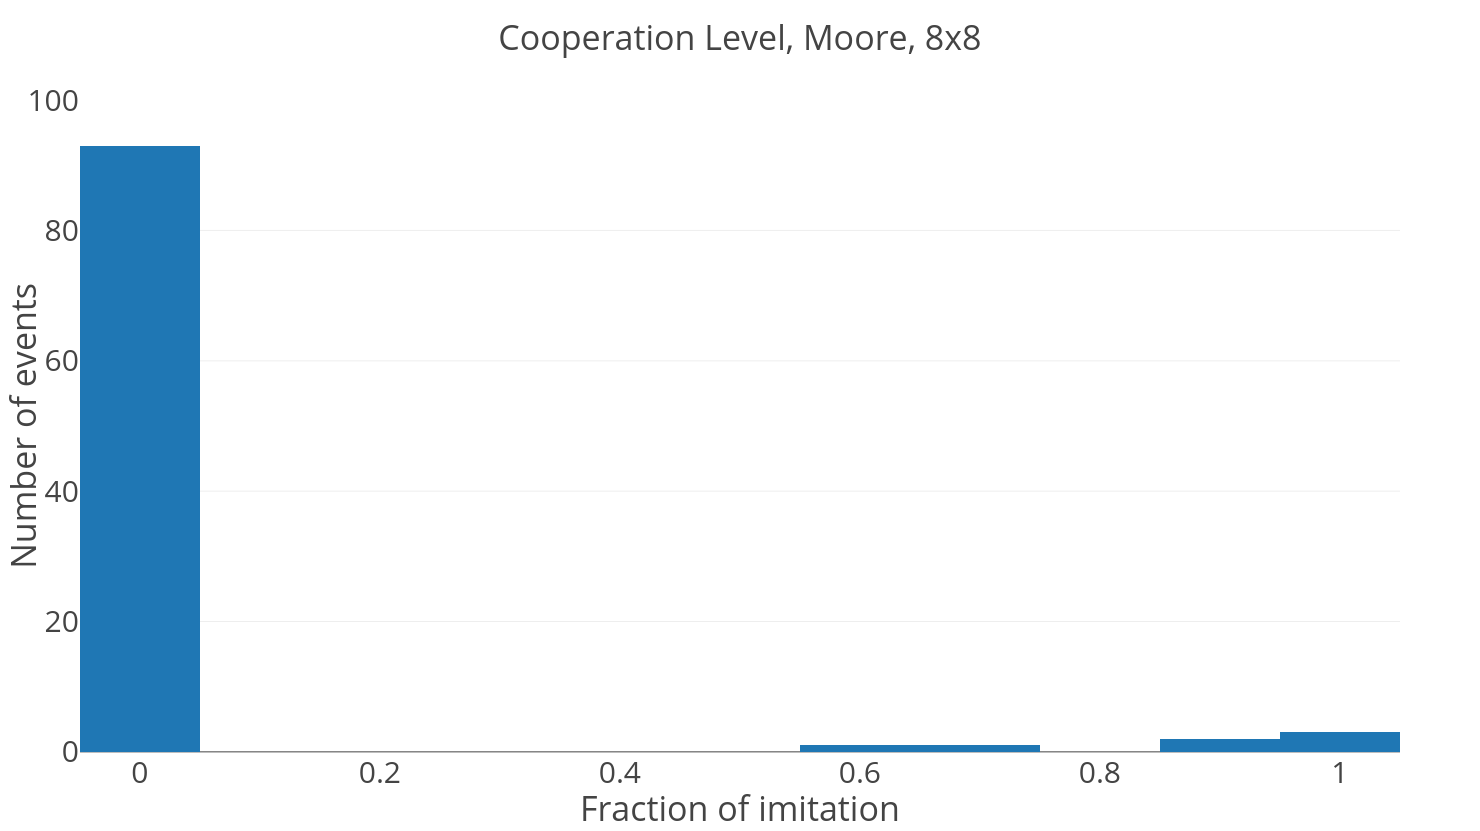
\includegraphics[width=1\linewidth]{PDMoore8x8HG}
\end{subfigure}%
\begin{subfigure}{.25\textwidth}
	mean = $0.0605$
	
	deviation = $0.2251$
\end{subfigure}

\end{figure}

Increasing the lattice to 8x8, we get our first pure cooperation and mixed strategy fields. The configuration converges after 4 rounds, but most fields end up as being pure defector lattices.

\newpage

%%%% 12x12
%%%%%%%%%%%%%%%%%%%%%%%%%%%%%%%%%%%%%%%%%
\subsubsection{12x12}
\begin{figure}[H]
\centering
\begin{subfigure}{.16\textwidth}
  \centering
  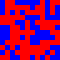
\includegraphics[width=0.9\linewidth]{PRISONERS_DILEMMA_MOORE_12x12_t00}
  \caption{t=0}
\end{subfigure}%
\begin{subfigure}{.16\textwidth}
  \centering
  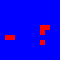
\includegraphics[width=0.9\linewidth]{PRISONERS_DILEMMA_MOORE_12x12_t01}
  \caption{t=1}
\end{subfigure}%
\begin{subfigure}{.16\textwidth}
  \centering
  
\includegraphics[width=0.9\linewidth]{PRISONERS_DILEMMA_MOORE_12x12_t05}
  \caption{t=5}
\end{subfigure}%
\begin{subfigure}{.16\textwidth}
  \centering
  
\includegraphics[width=0.9\linewidth]{PRISONERS_DILEMMA_MOORE_12x12_t10}
  \caption{t=10}
\end{subfigure}%
\begin{subfigure}{.16\textwidth}
  \centering
  
\includegraphics[width=0.9\linewidth]{PRISONERS_DILEMMA_MOORE_12x12_t20}
  \caption{t=20}
\end{subfigure}%
\begin{subfigure}{.16\textwidth}
  \centering
  
\includegraphics[width=0.9\linewidth]{PRISONERS_DILEMMA_MOORE_12x12_t50}
  \caption{t=50}
\end{subfigure}
\caption{Prisoners Dilemma, Moore, 12x12}
\end{figure}


\begin{figure}[H]
\begin{subfigure}{.75\textwidth}
	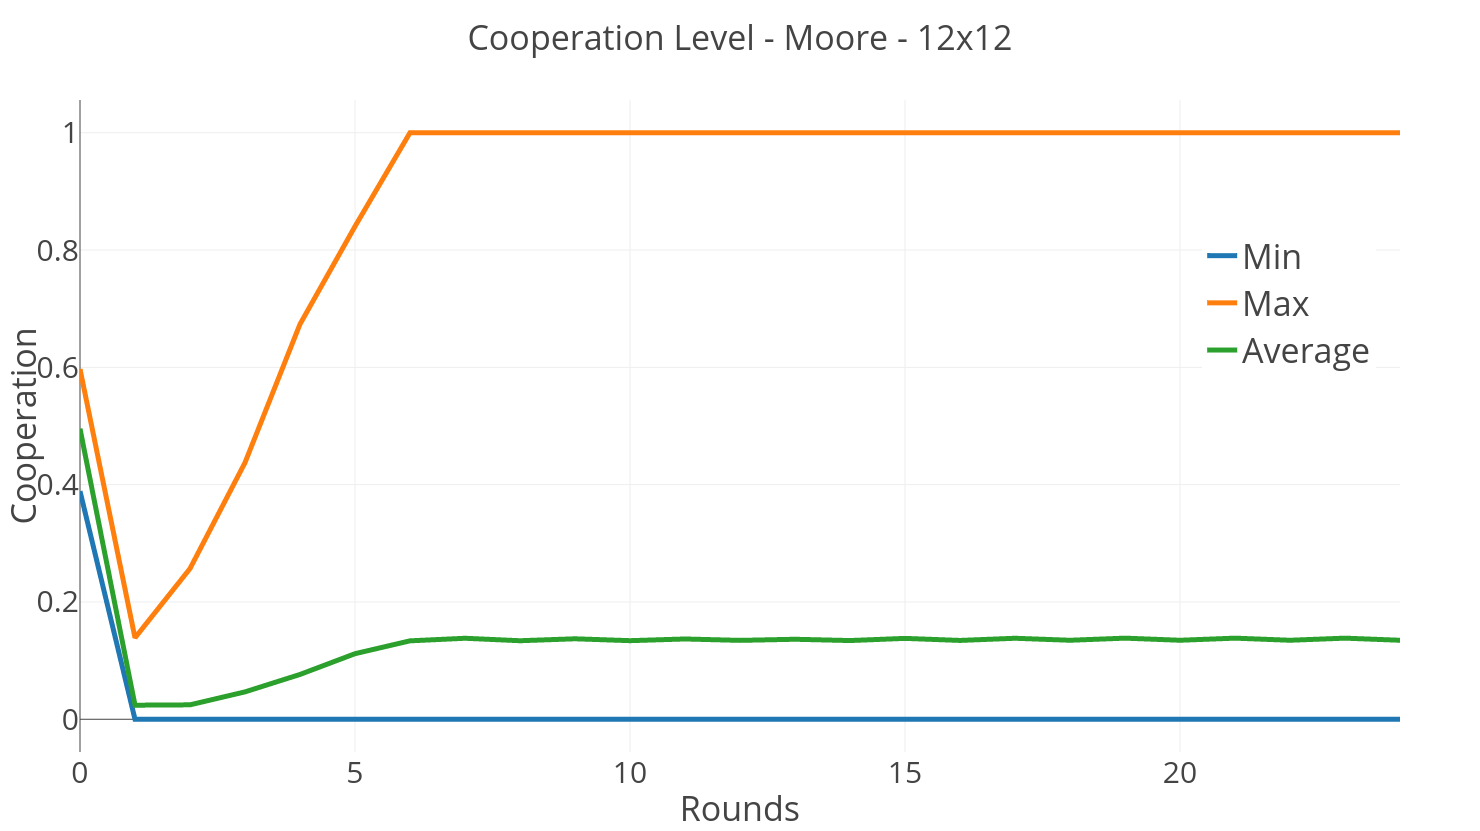
\includegraphics[width=1\linewidth]{PDMoore12x12}
\end{subfigure}

\begin{subfigure}{.75\textwidth}
	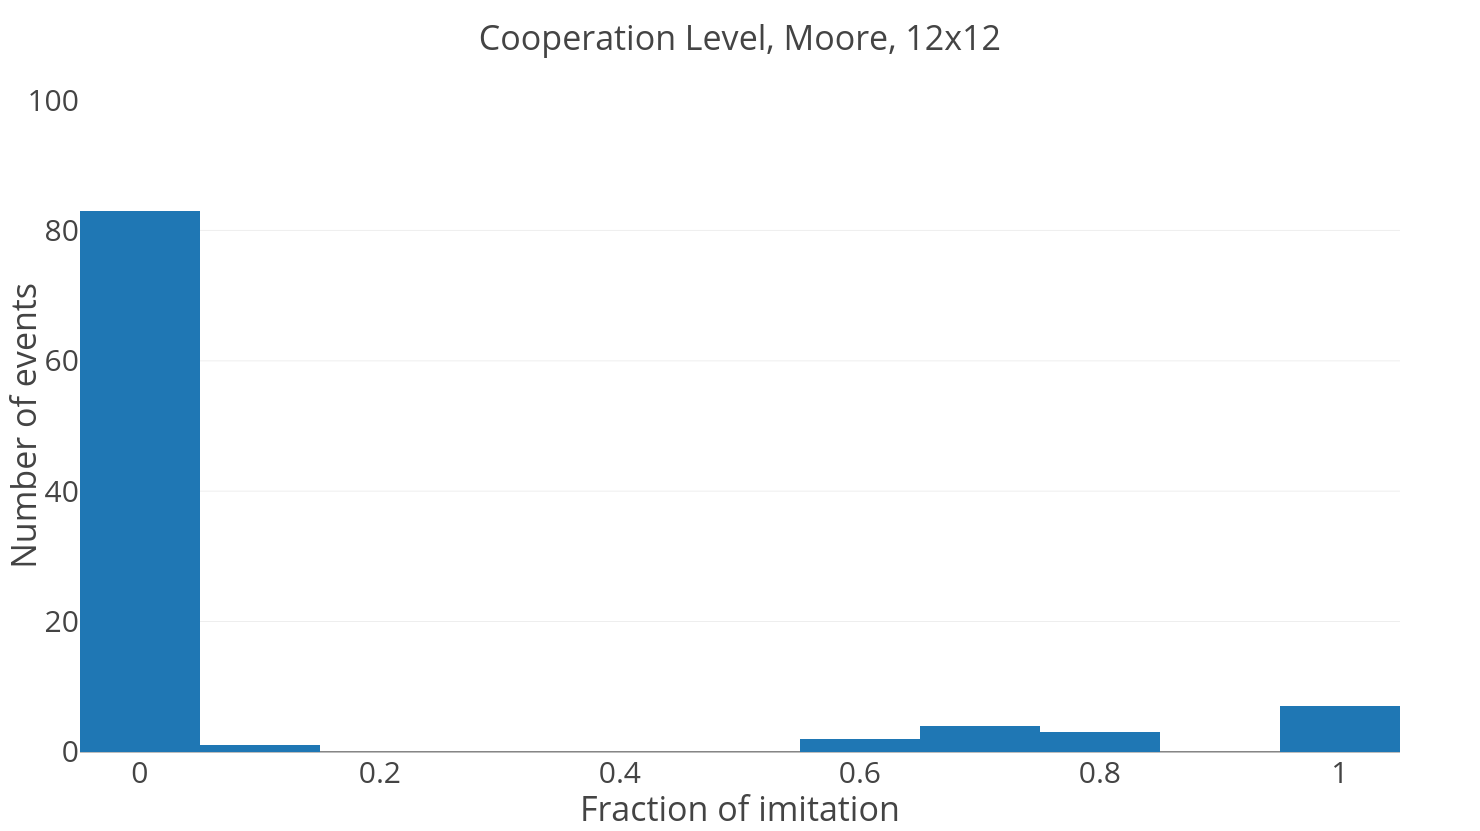
\includegraphics[width=1\linewidth]{PDMoore12x12HG}
\end{subfigure}%
\begin{subfigure}{.25\textwidth}
	mean = $0.1347$
	
	deviation = $0.3115$
\end{subfigure}

\end{figure}

A lattice configuration of 12x12 increases the chance slightly that the whole lattice does not end up being only defectors. More mixed strategy lattices at $0.7$ and some more pure strategy cooperation lattices. Convergence after 7 rounds.

\newpage

%%%% 20x20
%%%%%%%%%%%%%%%%%%%%%%%%%%%%%%%%%%%%%%%%%
\subsubsection{20x20}
\begin{figure}[H]
\centering
\begin{subfigure}{.16\textwidth}
  \centering
  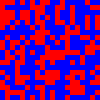
\includegraphics[width=0.9\linewidth]{PRISONERS_DILEMMA_MOORE_20x20_t00}
  \caption{t=0}
\end{subfigure}%
\begin{subfigure}{.16\textwidth}
  \centering
  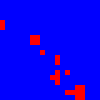
\includegraphics[width=0.9\linewidth]{PRISONERS_DILEMMA_MOORE_20x20_t01}
  \caption{t=1}
\end{subfigure}%
\begin{subfigure}{.16\textwidth}
  \centering
  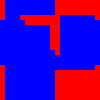
\includegraphics[width=0.9\linewidth]{PRISONERS_DILEMMA_MOORE_20x20_t05}
  \caption{t=5}
\end{subfigure}
\begin{subfigure}{.16\textwidth}
  \centering
  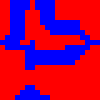
\includegraphics[width=0.9\linewidth]{PRISONERS_DILEMMA_MOORE_20x20_t10}
  \caption{t=10}
\end{subfigure}%
\begin{subfigure}{.16\textwidth}
  \centering
  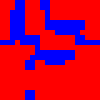
\includegraphics[width=0.9\linewidth]{PRISONERS_DILEMMA_MOORE_20x20_t20}
  \caption{t=20}
\end{subfigure}%
\begin{subfigure}{.16\textwidth}
  \centering
  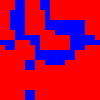
\includegraphics[width=0.9\linewidth]{PRISONERS_DILEMMA_MOORE_20x20_t50}
  \caption{t=50}
\end{subfigure}
\caption{Prisoners Dilemma, Moore, 20x20}
\end{figure}

\begin{figure}[H]
\begin{subfigure}{.75\textwidth}
	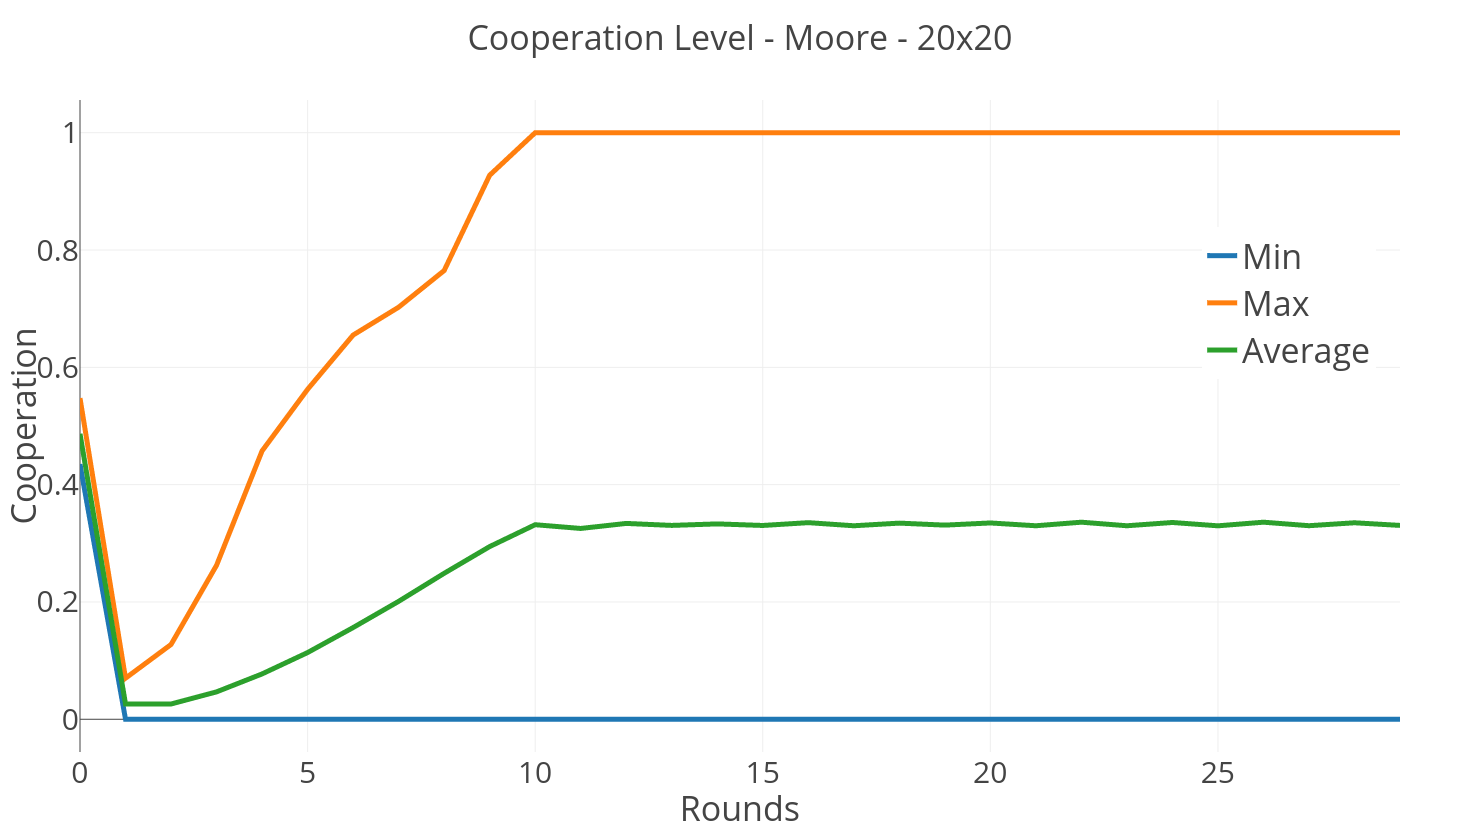
\includegraphics[width=1\linewidth]{PDMoore20x20}
\end{subfigure}

\begin{subfigure}{.75\textwidth}
	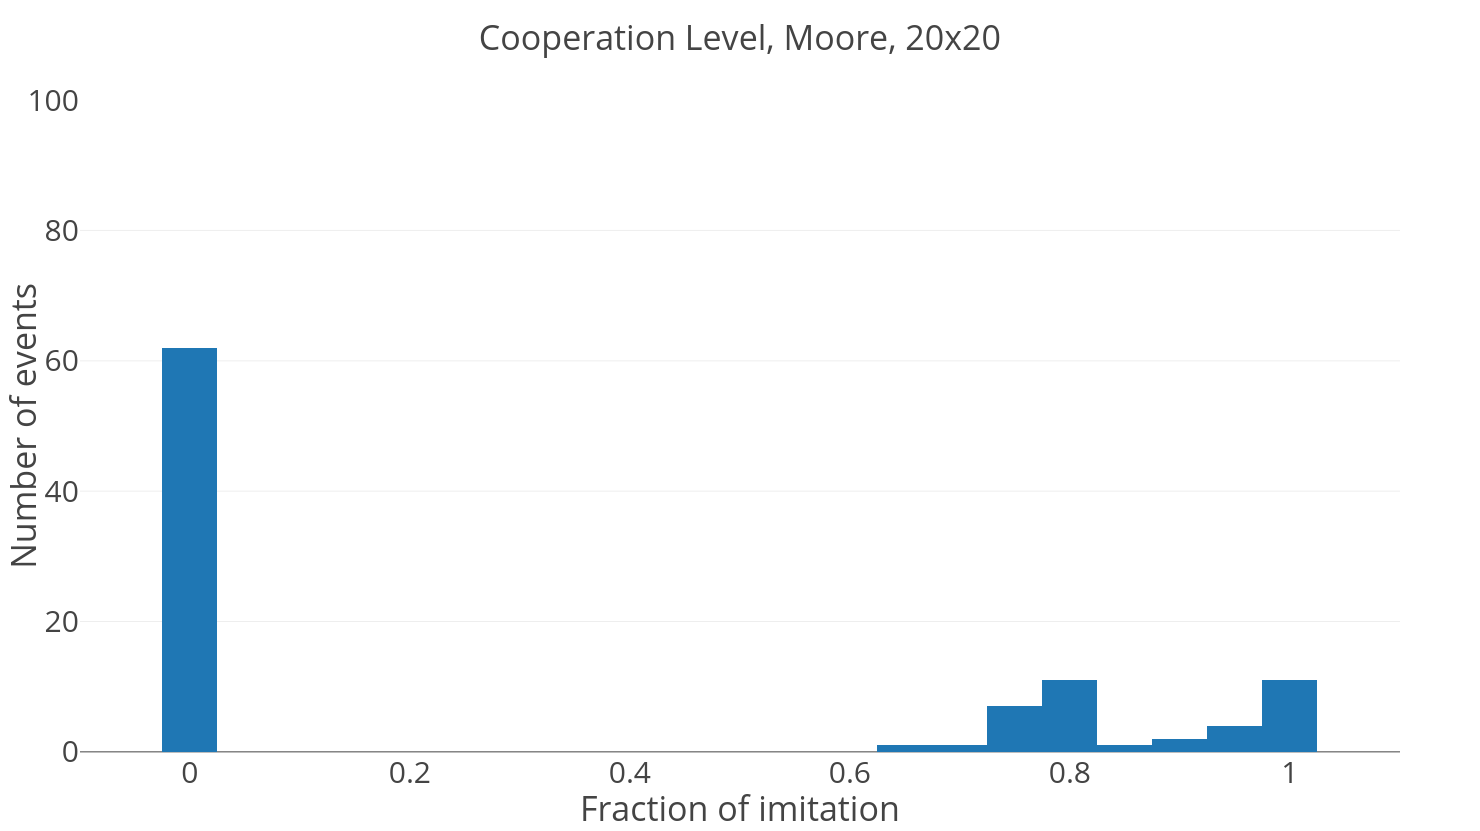
\includegraphics[width=1\linewidth]{PDMoore20x20HG}
\end{subfigure}%
\begin{subfigure}{.25\textwidth}
	mean = $0.3305$
	
	deviation = $0.4262$
\end{subfigure}

\end{figure}

The 20x20 lattice configuration results in $60 \%$ of games being purely defectors and the rest being either purely cooperative or mostly cooperative. The graphical representation shows the creation of cooperation blocks after time, with defector \textit{rivers} in between. 


\newpage
%%%% 50x50
%%%%%%%%%%%%%%%%%%%%%%%%%%%%%%%%%%%%%%%%%
\subsubsection{50x50}
\begin{figure}[H]
\centering
\begin{subfigure}{.16\textwidth}
  \centering
  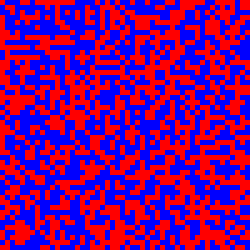
\includegraphics[width=0.9\linewidth]{PRISONERS_DILEMMA_MOORE_50x50_t00}
  \caption{t=0}
\end{subfigure}%
\begin{subfigure}{.16\textwidth}
  \centering
  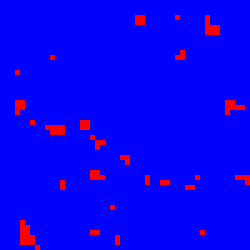
\includegraphics[width=0.9\linewidth]{PRISONERS_DILEMMA_MOORE_50x50_t01}
  \caption{t=1}
\end{subfigure}%
\begin{subfigure}{.16\textwidth}
  \centering
  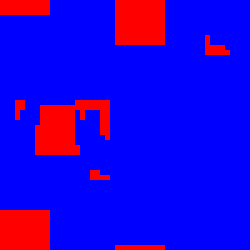
\includegraphics[width=0.9\linewidth]{PRISONERS_DILEMMA_MOORE_50x50_t05}
  \caption{t=5}
\end{subfigure}
\begin{subfigure}{.16\textwidth}
  \centering
  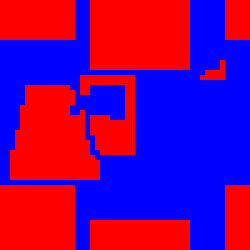
\includegraphics[width=0.9\linewidth]{PRISONERS_DILEMMA_MOORE_50x50_t10}
  \caption{t=10}
\end{subfigure}%
\begin{subfigure}{.16\textwidth}
  \centering
  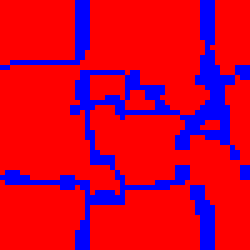
\includegraphics[width=0.9\linewidth]{PRISONERS_DILEMMA_MOORE_50x50_t20}
  \caption{t=20}
\end{subfigure}%
\begin{subfigure}{.16\textwidth}
  \centering
  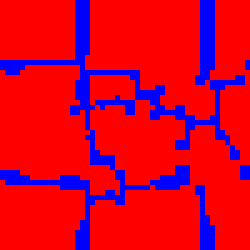
\includegraphics[width=0.9\linewidth]{PRISONERS_DILEMMA_MOORE_50x50_t50}
  \caption{t=50}
\end{subfigure}
\caption{Prisoners Dilemma, Moore, 50x50}
\end{figure}

\begin{figure}[H]
\begin{subfigure}{.75\textwidth}
	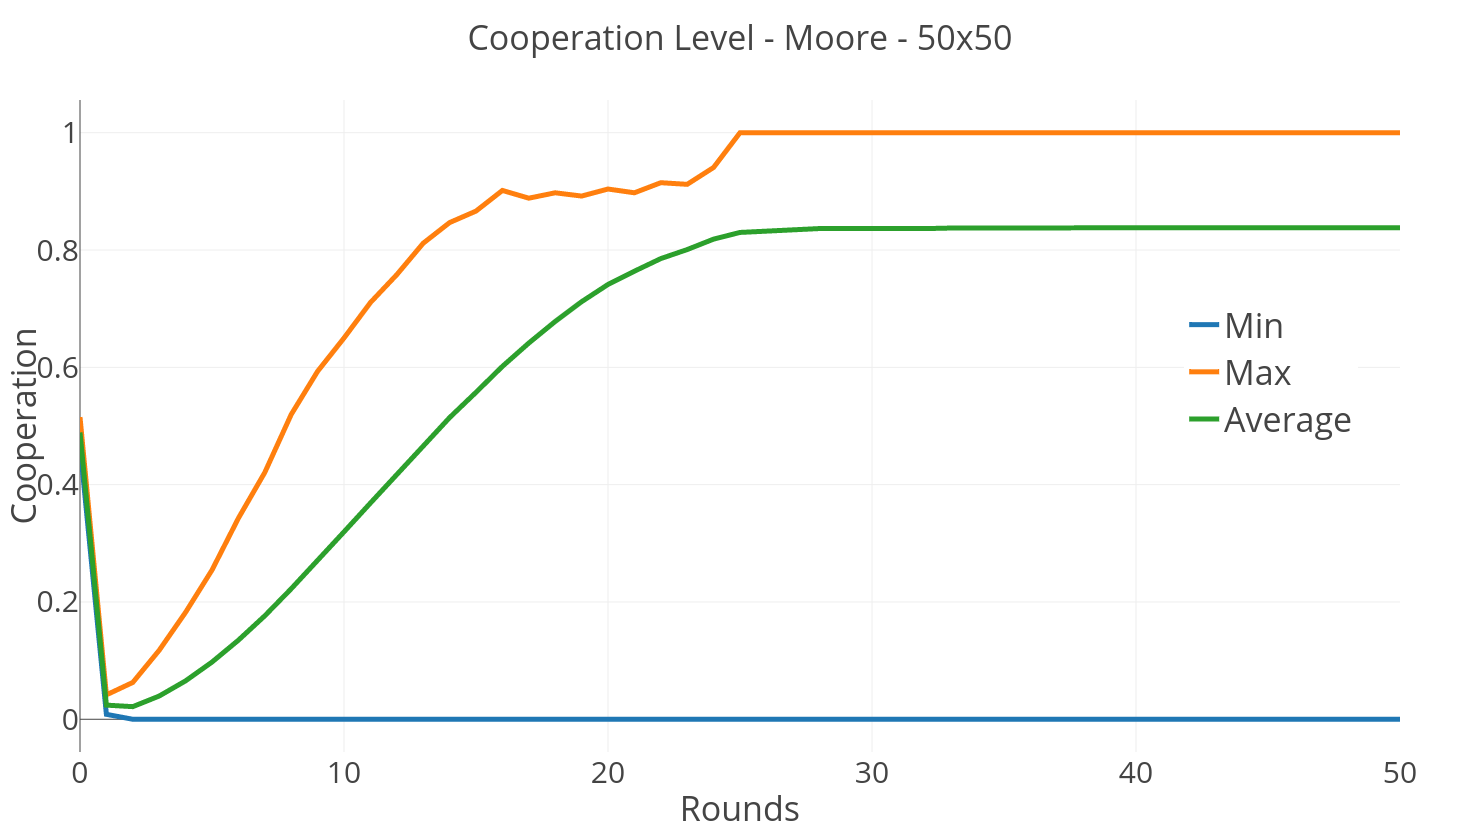
\includegraphics[width=1\linewidth]{PDMoore50x50}
\end{subfigure}

\begin{subfigure}{.75\textwidth}
	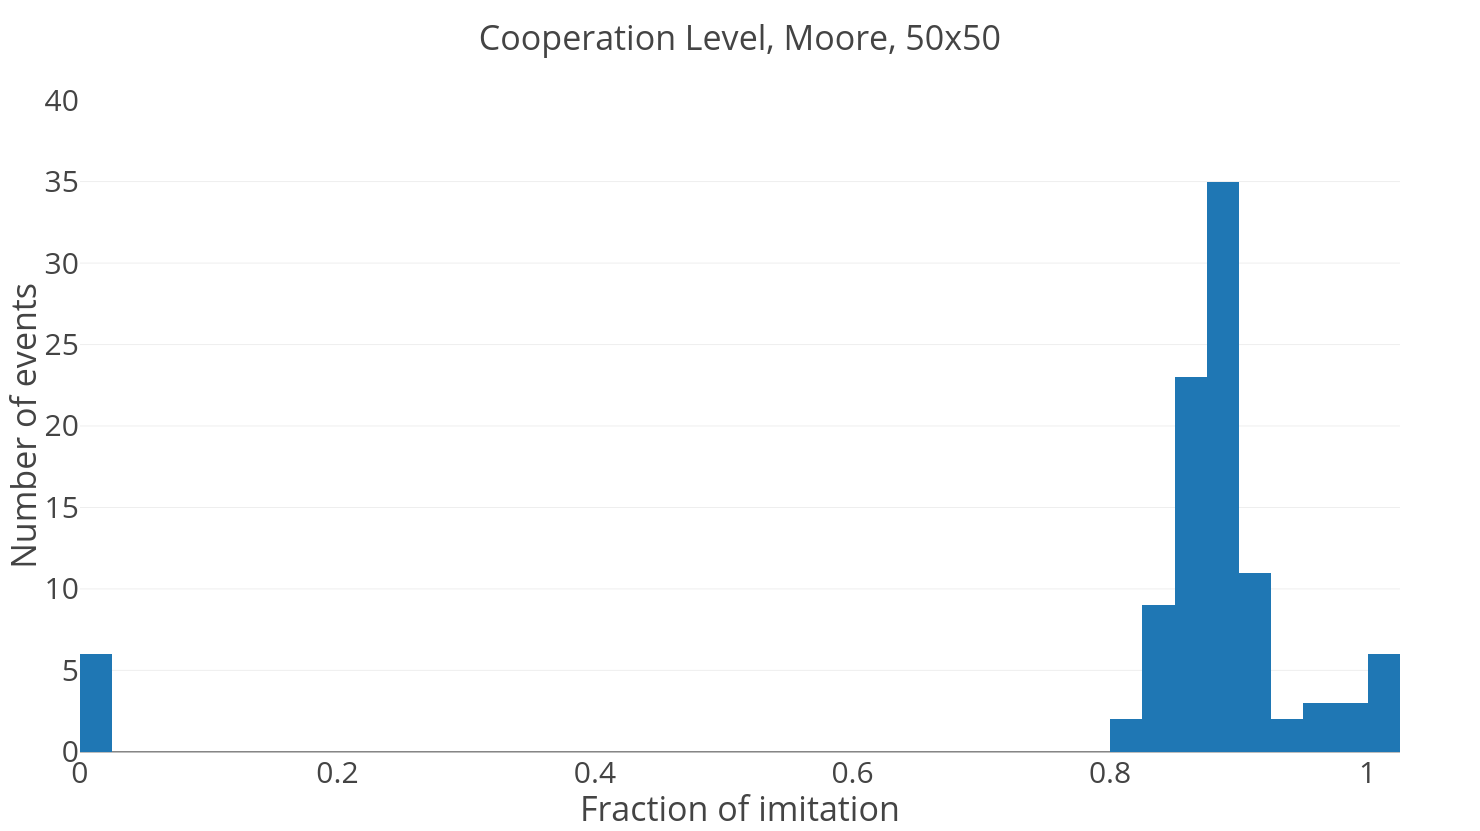
\includegraphics[width=1\linewidth]{PDMoore50x50HG}
\end{subfigure}%
\begin{subfigure}{.25\textwidth}
	mean = $0.8379$
	
	deviation = $0.2165$
\end{subfigure}

\end{figure}

A 50x50 lattice configuration results in a highly cooperative environment about $94\%$ of the time. Convergence after 25 rounds. Looking at the graphical representation we can see that clusters of cooperation with \textit{rivers} of defection are being formed. The distribution starts to look like a normal distribution.

\newpage

%%%%%%%%%%%%%%%%%%%%%%%%%
\subsection{Von Neumann Neighborhood}

\subsubsection{50x50}
\begin{figure}[H]
\centering
\begin{subfigure}{.25\textwidth}
  \centering
  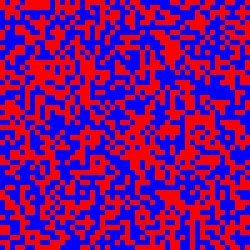
\includegraphics[width=0.9\linewidth]{PRISONERS_DILEMMA_VON_NEUMANN_50x50_t00}
  \caption{t=0}
\end{subfigure}%
\begin{subfigure}{.25\textwidth}
  \centering
  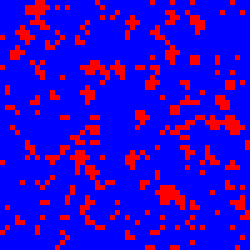
\includegraphics[width=0.9\linewidth]{PRISONERS_DILEMMA_VON_NEUMANN_50x50_t01}
  \caption{t=1}
\end{subfigure}%
\begin{subfigure}{.25\textwidth}
  \centering
  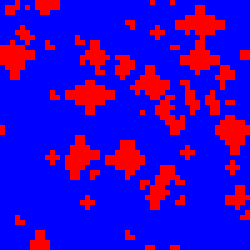
\includegraphics[width=0.9\linewidth]{PRISONERS_DILEMMA_VON_NEUMANN_50x50_t05}
  \caption{t=5}
\end{subfigure}%
\begin{subfigure}{.25\textwidth}
  \centering
  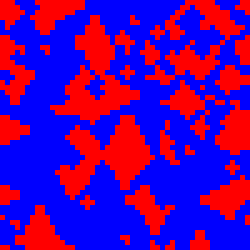
\includegraphics[width=0.9\linewidth]{PRISONERS_DILEMMA_VON_NEUMANN_50x50_t10}
  \caption{t=10}
\end{subfigure}
\begin{subfigure}{.25\textwidth}
  \centering
  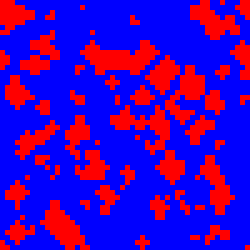
\includegraphics[width=0.9\linewidth]{PRISONERS_DILEMMA_VON_NEUMANN_50x50_t20}
  \caption{t=20}
\end{subfigure}%
\begin{subfigure}{.25\textwidth}
  \centering
  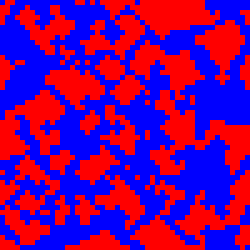
\includegraphics[width=0.9\linewidth]{PRISONERS_DILEMMA_VON_NEUMANN_50x50_t50}
  \caption{t=50}
\end{subfigure}%
\begin{subfigure}{.25\textwidth}
  \centering
  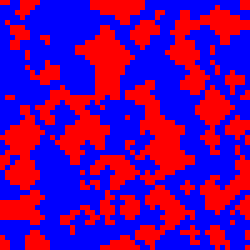
\includegraphics[width=0.9\linewidth]{PRISONERS_DILEMMA_VON_NEUMANN_50x50_t75}
  \caption{t=75}
\end{subfigure}%
\begin{subfigure}{.25\textwidth}
  \centering
  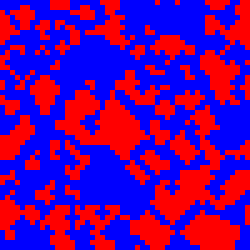
\includegraphics[width=0.9\linewidth]{PRISONERS_DILEMMA_VON_NEUMANN_50x50_t100}
  \caption{t=100}
\end{subfigure}
\caption{Prisoners Dilemma, Von Neumann, 50x50}
\end{figure}


\begin{figure}[H]
\begin{subfigure}{.55\textwidth}
	\begin{subfigure}{1\textwidth}
		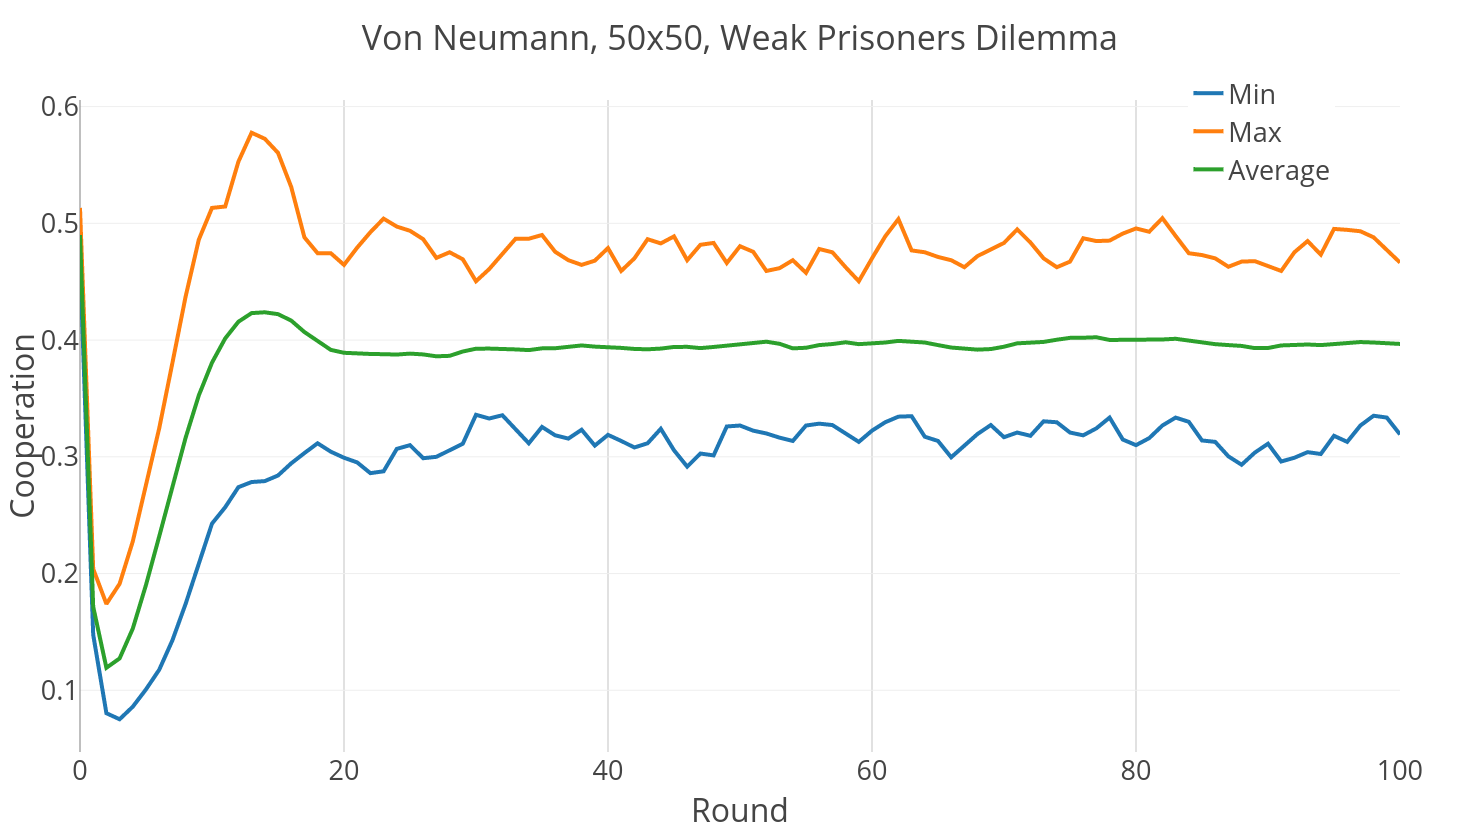
\includegraphics[width=1\linewidth]{PDVonNeumann50x50}
	\end{subfigure}

	\begin{subfigure}{1\textwidth}
		\includegraphics[width=1\linewidth]{PDVonNeumann50x50HG}
	\end{subfigure}
\end{subfigure}%
\begin{subfigure}{.45\textwidth}
	Changing the neighborhood to the \textit{Von Neumann} mode, we get a mean = $0.3914$ and deviation = $0.0263$. The mean with this neighborhood type is about half as the mean from a Moore neighborhood game with the same lattice size. The deviation is however much smaller.
	
	The configuration converges after 20 rounds. Looking at the differences of the graphical representation, using the Von Neumann neighborhood results in non stationary clusters as we have with a Moore neighborhood. The cooperation level over time also changes, which we can observe in the curve. It does not drop too much at the first few rounds and then quickly converges to $\sim 0.4\%$ with the maximum and minimum level not being too far away which is why the deviation is much smaller compared to the Moore neighborhood. This is because of the influence caused by the defector players in the first few rounds is reduced with fewer neighbors.
	
	
\end{subfigure}

\end{figure}


\newpage
\subsection{Analysing the results}

We can now have a look at the results of the experiments and investigate their differences.

\begin{table}[H]
\centering
\caption{Combined Experiment Results}
\begin{tabular}{l|l|l|l|l|l|l|l}
            & \multicolumn{5}{c|}{Moore}              & Von Neumann &  \\ \cline{1-7}
Lattice     & 4x4 & 8x8    & 12x12  & 20x20  & 50x50  & 50x50       &  \\ \cline{1-7}
Mean        & 0   & 0.0605 & 0.1347 & 0.3305 & 0.8379 & 0.3914      &  \\ \cline{1-7}
Deviation   & 0   & 0.2251 & 0.3115 & 0.4262 & 0.2165 & 0.0263      &  \\ \cline{1-7}
Convergence & 3   & 4      & 7      & 10     & 25     & 20          &  \\ \cline{1-7}
\end{tabular}
\end{table}

Looking only at the Moore neighborhood configurations, we can observe that the mean increases and the deviation decreases with an increase in the lattice size. Lattices that converge with cooperation blocks divided by defector \textit{rivers} do need a large lattice size to occur regularly - this shown by the increase of the mean. The time to converge to a constant level does depend on the lattice size according to our results - the bigger the size, the higher the time to converge.




%%%%%%%%%%%%%%%%%%%%%%%%%%%%%%%%%%%%%%%%%%%%%%%%
%%%%%%%%%%%%%%%%%%%%%%%%%%%%%%%%%%%%%%%%%%%%%%%%
%%%%%%%%%%%%%%%%%%%%%%%%%%%%%%%%%%%%%%%%%%%%%%%%

\hrule

\section{Part Two - Spatial Snowdrift Game - Replicator Rule}

Replicator rule

\[ P_{ij} = \frac{1+ \frac{W_j-W_i}{N \times (max\{P,R,T,S\} - min\{P,R,T,S\})}}{2} \]

With the Snowdrift game, this formula becomes

\[ P_{ij} = \frac{1+ \frac{W_j-W_i}{80}}{2} \]

with the Moore neighborhood or

\[ P_{ij} = \frac{1+ \frac{W_j-W_i}{40}}{2} \]

with the Von Neumann neighborhood. This probabilistic method assures enables a \textit{mixed} strategy of replicating. Contrary to a \textit{pure} strategy as experimented with in part one, the replicator rule assigns a probability of choosing the strategy of the other player by taking the difference of the payoff between the two players. The greater the difference of $W_j - W_i$, the more likely it is to replicate the action

The $N$ variable reduces this probability - more neighbors lead to a slightly smaller probability of replicating the opponent strategy. It makes sense to have a probabilistic update mechanism as many real \textit{games} have mixed strategies instead of pure ones - it allows for the modelling of phenomena’s we can see in nature for example.



\newpage

%%%%%%%%%%%%%%%%%%%%%%%%%
\subsection{Moore Neighborhood}

\subsubsection{4x4}
\begin{figure}[H]
\centering
\begin{subfigure}{.25\textwidth}
  \centering
  \includegraphics[width=0.9\linewidth]{SNOWDRIFT_MOORE_4x4_t00}
  \caption{t=0}
\end{subfigure}%
\begin{subfigure}{.25\textwidth}
  \centering
  \includegraphics[width=0.9\linewidth]{SNOWDRIFT_MOORE_4x4_t01}
  \caption{t=1}
\end{subfigure}%
\begin{subfigure}{.25\textwidth}
  \centering
  \includegraphics[width=0.9\linewidth]{SNOWDRIFT_MOORE_4x4_t05}
  \caption{t=5}
\end{subfigure}%
\begin{subfigure}{.25\textwidth}
  \centering
  \includegraphics[width=0.9\linewidth]{SNOWDRIFT_MOORE_4x4_t10}
  \caption{t=10}
\end{subfigure}
\begin{subfigure}{.25\textwidth}
  \centering
  \includegraphics[width=0.9\linewidth]{SNOWDRIFT_MOORE_4x4_t20}
  \caption{t=20}
\end{subfigure}%
\begin{subfigure}{.25\textwidth}
  \centering
  \includegraphics[width=0.9\linewidth]{SNOWDRIFT_MOORE_4x4_t50}
  \caption{t=50}
\end{subfigure}%
\begin{subfigure}{.25\textwidth}
  \centering
  \includegraphics[width=0.9\linewidth]{SNOWDRIFT_MOORE_4x4_t75}
  \caption{t=75}
\end{subfigure}%
\begin{subfigure}{.25\textwidth}
  \centering
  \includegraphics[width=0.9\linewidth]{SNOWDRIFT_MOORE_4x4_t100}
  \caption{t=100}
\end{subfigure}
\caption{Snowdrift Game, Moore, 4x4}
\end{figure}


\begin{figure}[H]
\begin{subfigure}{.55\textwidth}
	\begin{subfigure}{1\textwidth}
		\includegraphics[width=1\linewidth]{SDMoore4x4}
	\end{subfigure}

	\begin{subfigure}{1\textwidth}
		\includegraphics[width=1\linewidth]{SDMoore4x4HG}
	\end{subfigure}
\end{subfigure}%
\begin{subfigure}{.45\textwidth}
	We get a mean = $0.4738$ and deviation = $0.1354$. The simulation converges after about 10 rounds. Contrary to the old update strategy, we don't have a single pure strategy lattice and the distribution looks already somewhat like a normal distribution.
\end{subfigure}

\end{figure}


\newpage
%%%%%%%%%%%%%%%%%%%%%%%%%

\subsubsection{8x8}
\begin{figure}[H]
\centering
\begin{subfigure}{.25\textwidth}
  \centering
  \includegraphics[width=0.9\linewidth]{SNOWDRIFT_MOORE_8x8_t00}
  \caption{t=0}
\end{subfigure}%
\begin{subfigure}{.25\textwidth}
  \centering
  \includegraphics[width=0.9\linewidth]{SNOWDRIFT_MOORE_8x8_t01}
  \caption{t=1}
\end{subfigure}%
\begin{subfigure}{.25\textwidth}
  \centering
  \includegraphics[width=0.9\linewidth]{SNOWDRIFT_MOORE_8x8_t05}
  \caption{t=5}
\end{subfigure}%
\begin{subfigure}{.25\textwidth}
  \centering
  \includegraphics[width=0.9\linewidth]{SNOWDRIFT_MOORE_8x8_t10}
  \caption{t=10}
\end{subfigure}
\begin{subfigure}{.25\textwidth}
  \centering
  \includegraphics[width=0.9\linewidth]{SNOWDRIFT_MOORE_8x8_t20}
  \caption{t=20}
\end{subfigure}%
\begin{subfigure}{.25\textwidth}
  \centering
  \includegraphics[width=0.9\linewidth]{SNOWDRIFT_MOORE_8x8_t50}
  \caption{t=50}
\end{subfigure}%
\begin{subfigure}{.25\textwidth}
  \centering
  \includegraphics[width=0.9\linewidth]{SNOWDRIFT_MOORE_8x8_t75}
  \caption{t=75}
\end{subfigure}%
\begin{subfigure}{.25\textwidth}
  \centering
  \includegraphics[width=0.9\linewidth]{SNOWDRIFT_MOORE_8x8_t100}
  \caption{t=100}
\end{subfigure}
\caption{Snowdrift Game, Moore, 8x8}
\end{figure}


\begin{figure}[H]
\begin{subfigure}{.55\textwidth}
	\begin{subfigure}{1\textwidth}
		\includegraphics[width=1\linewidth]{SDMoore8x8}
	\end{subfigure}

	\begin{subfigure}{1\textwidth}
		\includegraphics[width=1\linewidth]{SDMoore8x8HG}
	\end{subfigure}
\end{subfigure}%
\begin{subfigure}{.45\textwidth}
	Again no pure strategy lattice and we get a mean = $0.4658$ and deviation = $0.0698$. A reduction in the deviation from the previous lattice size. The simulation converges at about the same time, after 10 rounds.
\end{subfigure}

\end{figure}



\newpage
%%%%%%%%%%%%%%%%%%%%%%%%%

\subsubsection{12x12}
\begin{figure}[H]
\centering
\begin{subfigure}{.25\textwidth}
  \centering
  \includegraphics[width=0.9\linewidth]{SNOWDRIFT_MOORE_12x12_t00}
  \caption{t=0}
\end{subfigure}%
\begin{subfigure}{.25\textwidth}
  \centering
  \includegraphics[width=0.9\linewidth]{SNOWDRIFT_MOORE_12x12_t01}
  \caption{t=1}
\end{subfigure}%
\begin{subfigure}{.25\textwidth}
  \centering
  \includegraphics[width=0.9\linewidth]{SNOWDRIFT_MOORE_12x12_t05}
  \caption{t=5}
\end{subfigure}%
\begin{subfigure}{.25\textwidth}
  \centering
  \includegraphics[width=0.9\linewidth]{SNOWDRIFT_MOORE_12x12_t10}
  \caption{t=10}
\end{subfigure}
\begin{subfigure}{.25\textwidth}
  \centering
  \includegraphics[width=0.9\linewidth]{SNOWDRIFT_MOORE_12x12_t20}
  \caption{t=20}
\end{subfigure}%
\begin{subfigure}{.25\textwidth}
  \centering
  \includegraphics[width=0.9\linewidth]{SNOWDRIFT_MOORE_12x12_t50}
  \caption{t=50}
\end{subfigure}%
\begin{subfigure}{.25\textwidth}
  \centering
  \includegraphics[width=0.9\linewidth]{SNOWDRIFT_MOORE_12x12_t75}
  \caption{t=75}
\end{subfigure}%
\begin{subfigure}{.25\textwidth}
  \centering
  \includegraphics[width=0.9\linewidth]{SNOWDRIFT_MOORE_12x12_t100}
  \caption{t=100}
\end{subfigure}
\caption{Snowdrift Game, Moore, 12x12}
\end{figure}


\begin{figure}[H]
\begin{subfigure}{.55\textwidth}
	\begin{subfigure}{1\textwidth}
		\includegraphics[width=1\linewidth]{SDMoore12x12}
	\end{subfigure}

	\begin{subfigure}{1\textwidth}
		\includegraphics[width=1\linewidth]{SDMoore12x12HG}
	\end{subfigure}
\end{subfigure}%
\begin{subfigure}{.45\textwidth}
	Mean = $0.4682$ and deviation = $0.0384$. Convergence also after about 10 rounds. Also a reduction in the deviation, but the mean stays at the same level.
\end{subfigure}

\end{figure}




\newpage
%%%%%%%%%%%%%%%%%%%%%%%%%

\subsubsection{20x20}
\begin{figure}[H]
\centering
\begin{subfigure}{.25\textwidth}
  \centering
  \includegraphics[width=0.9\linewidth]{SNOWDRIFT_MOORE_20x20_t00}
  \caption{t=0}
\end{subfigure}%
\begin{subfigure}{.25\textwidth}
  \centering
  \includegraphics[width=0.9\linewidth]{SNOWDRIFT_MOORE_20x20_t01}
  \caption{t=1}
\end{subfigure}%
\begin{subfigure}{.25\textwidth}
  \centering
  \includegraphics[width=0.9\linewidth]{SNOWDRIFT_MOORE_20x20_t05}
  \caption{t=5}
\end{subfigure}%
\begin{subfigure}{.25\textwidth}
  \centering
  \includegraphics[width=0.9\linewidth]{SNOWDRIFT_MOORE_20x20_t10}
  \caption{t=10}
\end{subfigure}
\begin{subfigure}{.25\textwidth}
  \centering
  \includegraphics[width=0.9\linewidth]{SNOWDRIFT_MOORE_20x20_t20}
  \caption{t=20}
\end{subfigure}%
\begin{subfigure}{.25\textwidth}
  \centering
  \includegraphics[width=0.9\linewidth]{SNOWDRIFT_MOORE_20x20_t50}
  \caption{t=50}
\end{subfigure}%
\begin{subfigure}{.25\textwidth}
  \centering
  \includegraphics[width=0.9\linewidth]{SNOWDRIFT_MOORE_20x20_t75}
  \caption{t=75}
\end{subfigure}%
\begin{subfigure}{.25\textwidth}
  \centering
  \includegraphics[width=0.9\linewidth]{SNOWDRIFT_MOORE_20x20_t100}
  \caption{t=100}
\end{subfigure}
\caption{Snowdrift Game, Moore, 20x20}
\end{figure}


\begin{figure}[H]
\begin{subfigure}{.55\textwidth}
	\begin{subfigure}{1\textwidth}
		\includegraphics[width=1\linewidth]{SDMoore20x20}
	\end{subfigure}

	\begin{subfigure}{1\textwidth}
		\includegraphics[width=1\linewidth]{SDMoore20x20HG}
	\end{subfigure}
\end{subfigure}%
\begin{subfigure}{.45\textwidth}
	Mean = $0.4711$ and deviation = $0.0239$. The trend continues: lower deviation, convergence after about 10 rounds. Comparing this lattice size to the old update mechanism, we don't observe the cooperative block creation.
\end{subfigure}

\end{figure}





\newpage
%%%%%%%%%%%%%%%%%%%%%%%%%

\subsubsection{50x50}
\begin{figure}[H]
\centering
\begin{subfigure}{.25\textwidth}
  \centering
  \includegraphics[width=0.9\linewidth]{SNOWDRIFT_MOORE_50x50_t00}
  \caption{t=0}
\end{subfigure}%
\begin{subfigure}{.25\textwidth}
  \centering
  \includegraphics[width=0.9\linewidth]{SNOWDRIFT_MOORE_50x50_t01}
  \caption{t=1}
\end{subfigure}%
\begin{subfigure}{.25\textwidth}
  \centering
  \includegraphics[width=0.9\linewidth]{SNOWDRIFT_MOORE_50x50_t05}
  \caption{t=5}
\end{subfigure}%
\begin{subfigure}{.25\textwidth}
  \centering
  \includegraphics[width=0.9\linewidth]{SNOWDRIFT_MOORE_50x50_t10}
  \caption{t=10}
\end{subfigure}
\begin{subfigure}{.25\textwidth}
  \centering
  \includegraphics[width=0.9\linewidth]{SNOWDRIFT_MOORE_50x50_t20}
  \caption{t=20}
\end{subfigure}%
\begin{subfigure}{.25\textwidth}
  \centering
  \includegraphics[width=0.9\linewidth]{SNOWDRIFT_MOORE_50x50_t50}
  \caption{t=50}
\end{subfigure}%
\begin{subfigure}{.25\textwidth}
  \centering
  \includegraphics[width=0.9\linewidth]{SNOWDRIFT_MOORE_50x50_t75}
  \caption{t=75}
\end{subfigure}%
\begin{subfigure}{.25\textwidth}
  \centering
  \includegraphics[width=0.9\linewidth]{SNOWDRIFT_MOORE_50x50_t100}
  \caption{t=100}
\end{subfigure}
\caption{Snowdrift Game, Moore, 50x50}
\end{figure}


\begin{figure}[H]
\begin{subfigure}{.55\textwidth}
	\begin{subfigure}{1\textwidth}
		\includegraphics[width=1\linewidth]{SDMoore50x50}
	\end{subfigure}

	\begin{subfigure}{1\textwidth}
		\includegraphics[width=1\linewidth]{SDMoore50x50HG}
	\end{subfigure}
\end{subfigure}%
\begin{subfigure}{.45\textwidth}
	Mean = $0.473$ and deviation = $0.0117$. Same observation as previous lattice size. In the graphical representation we can observe that no stationary blocks are being formed.
\end{subfigure}

\end{figure}




\newpage

%%%%%%%%%%%%%%%%%%%%%%%%%
\subsection{Von Neumann Neighborhood}

\subsubsection{50x50}
\begin{figure}[H]
\centering
\begin{subfigure}{.25\textwidth}
  \centering
  \includegraphics[width=0.9\linewidth]{SNOWDRIFT_VON_NEUMANN_50x50_t00}
  \caption{t=0}
\end{subfigure}%
\begin{subfigure}{.25\textwidth}
  \centering
  \includegraphics[width=0.9\linewidth]{SNOWDRIFT_VON_NEUMANN_50x50_t01}
  \caption{t=1}
\end{subfigure}%
\begin{subfigure}{.25\textwidth}
  \centering
  \includegraphics[width=0.9\linewidth]{SNOWDRIFT_VON_NEUMANN_50x50_t05}
  \caption{t=5}
\end{subfigure}%
\begin{subfigure}{.25\textwidth}
  \centering
  \includegraphics[width=0.9\linewidth]{SNOWDRIFT_VON_NEUMANN_50x50_t10}
  \caption{t=10}
\end{subfigure}
\begin{subfigure}{.25\textwidth}
  \centering
  \includegraphics[width=0.9\linewidth]{SNOWDRIFT_VON_NEUMANN_50x50_t20}
  \caption{t=20}
\end{subfigure}%
\begin{subfigure}{.25\textwidth}
  \centering
  \includegraphics[width=0.9\linewidth]{SNOWDRIFT_VON_NEUMANN_50x50_t50}
  \caption{t=50}
\end{subfigure}%
\begin{subfigure}{.25\textwidth}
  \centering
  \includegraphics[width=0.9\linewidth]{SNOWDRIFT_VON_NEUMANN_50x50_t75}
  \caption{t=75}
\end{subfigure}%
\begin{subfigure}{.25\textwidth}
  \centering
  \includegraphics[width=0.9\linewidth]{SNOWDRIFT_VON_NEUMANN_50x50_t100}
  \caption{t=100}
\end{subfigure}
\caption{Snowdrift Game, Von Neumann, 50x50}
\end{figure}


\begin{figure}[H]
\begin{subfigure}{.55\textwidth}
	\begin{subfigure}{1\textwidth}
		\includegraphics[width=1\linewidth]{SDVonNeumann50x50}
	\end{subfigure}

	\begin{subfigure}{1\textwidth}
		\includegraphics[width=1\linewidth]{SDVonNeumann50x50HG}
	\end{subfigure}
\end{subfigure}%
\begin{subfigure}{.45\textwidth}
	Changing the neighborhood to the \textit{Von Neumann} mode, we get a mean = $0.4461$ and deviation = $0.0104$. Contrary to the observations of part one when changing the neighborhood type, we can not observe a large difference when changing to the Von Neumann method. The only difference is a slight reduction of the deviation
\end{subfigure}

\end{figure}



\newpage
\subsection{Analysing the results}

We can now have a combined look at the results of the experiments and investigate their differences.



\begin{table}[]
\centering
\caption{Combined Experiment Results}
\begin{tabular}{l|l|l|l|l|l|l|l}
            & \multicolumn{5}{c|}{Moore}                 & Von Neumann &  \\ \cline{1-7}
Lattice     & 4x4    & 8x8    & 12x12  & 20x20  & 50x50  & 50x50       &  \\ \cline{1-7}
Mean        & 0.4738 & 0.4658 & 0.4682 & 0.4711 & 0.473  & 0.4461      &  \\ \cline{1-7}
Deviation   & 0.1354 & 0.0698 & 0.0384 & 0.0239 & 0.0117 & 0.0104      &  \\ \cline{1-7}
Convergence & 10     & 10     & 10     & 10     & 10     & 10          &  \\ \cline{1-7}
\end{tabular}
\end{table}


From these results we can conclude that the mean stays relatively the same, no matter the lattice size. The deviation is being reduced with an increasing lattice size and the fields converge all at about the same number of rounds player: 10. Changing the neighborhood method to Von Neumann, the only difference we can observe is a slight reduction of the deviation.

\hrulefill


%%%%%%%%%%%%%%%%%%%%%%%%%%%%%%%%%%%%%%%%%%%%%%%%
%%%%%%%%%%%%%%%%%%%%%%%%%%%%%%%%%%%%%%%%%%%%%%%%
%%%%%%%%%%%%%%%%%%%%%%%%%%%%%%%%%%%%%%%%%%%%%%%%
\section{Part Three - Rock, Paper, Scissors}

For this extra part we will investigate a game with three actions: Rock, Paper, Scissors!

\begin{figure}[H]
  \begin{minipage}[b]{0.40\linewidth}
\includegraphics[width=1\linewidth]{Rock-paper-scissors}
\caption{Rock, Paper, Scissors}
  \end{minipage}%
  \begin{minipage}[b]{0.60\linewidth}
    \centering%
\begin{tabular}{cc|c|c|c|}
\cline{3-5}
                                                  &          & \multicolumn{3}{c|}{Player Two} \\ \cline{3-5} 
                                                  &          & Rock    & Paper    & Scissors   \\ \hline
\multicolumn{1}{|c|}{\multirow{3}{*}{Player One}} & Rock     & 0,0     & -1,1     & 1,-1       \\ \cline{2-5} 
\multicolumn{1}{|c|}{}                            & Paper    & 1,-1    & 0,0      & -1,1       \\ \cline{2-5} 
\multicolumn{1}{|c|}{}                            & Scissors & -1,1    & 1,-1     & 0,0        \\ \hline
\end{tabular}
\caption{Payoff Matrix}
    \par\vspace{0pt}
  \end{minipage}
\end{figure}


This game has a obvious mixed strategy Nash Equilibria with p(Rock)=p(Paper)=p(Scissors)=$\frac{1}{3}$. We shall investigate the effect of various starting population distributions and the effect this may have on the population of the lattice.

The following graphical lattice representation will use the following colors with the following actions:
\begin{itemize}[noitemsep]
  \item Rock - Red
  \item Paper - Blue
  \item Scissors - Green
\end{itemize}



\newpage
\begin{landscape}
\subsection{50x50, Equal starting distribution, Highest earner, Moore}

\begin{figure}[H]
\centering
\begin{subfigure}{.20\textwidth}
  \centering
  \includegraphics[width=0.95\linewidth]{ROCK_PAPER_SCISSORS_MOORE_50x50_t00}
  \caption{t=0}
\end{subfigure}%
\begin{subfigure}{.20\textwidth}
  \centering
  \includegraphics[width=0.95\linewidth]{ROCK_PAPER_SCISSORS_MOORE_50x50_t01}
  \caption{t=1}
\end{subfigure}%
\begin{subfigure}{.20\textwidth}
  \centering
  \includegraphics[width=0.95\linewidth]{ROCK_PAPER_SCISSORS_MOORE_50x50_t05}
  \caption{t=5}
\end{subfigure}%
\begin{subfigure}{.20\textwidth}
  \centering
  \includegraphics[width=0.95\linewidth]{ROCK_PAPER_SCISSORS_MOORE_50x50_t10}
  \caption{t=10}
\end{subfigure}%
\begin{subfigure}{.20\textwidth}
  \centering
  \includegraphics[width=0.95\linewidth]{ROCK_PAPER_SCISSORS_MOORE_50x50_t20}
  \caption{t=20}
\end{subfigure}%
\begin{subfigure}{.20\textwidth}
  \centering
  \includegraphics[width=0.95\linewidth]{ROCK_PAPER_SCISSORS_MOORE_50x50_t50}
  \caption{t=50}
\end{subfigure}%
\begin{subfigure}{.20\textwidth}
  \centering
  \includegraphics[width=0.95\linewidth]{ROCK_PAPER_SCISSORS_MOORE_50x50_t75}
  \caption{t=75}
\end{subfigure}%
\begin{subfigure}{.20\textwidth}
  \centering
  \includegraphics[width=0.95\linewidth]{ROCK_PAPER_SCISSORS_MOORE_50x50_t100}
  \caption{t=100}
\end{subfigure}
\caption{Rock - Paper - Scissors, Moore, 50x50}
\end{figure}


\begin{figure}[H]
	\begin{subfigure}{0.53\textwidth}
		\includegraphics[width=1\linewidth]{50x50_EqualDist_Rock}
		\caption{Rock population}
	\end{subfigure}%
	\begin{subfigure}{0.53\textwidth}
		\includegraphics[width=1\linewidth]{50x50_EqualDist_Paper}
		\caption{Paper population}
	\end{subfigure}%
	\begin{subfigure}{0.53\textwidth}
		\includegraphics[width=1\linewidth]{50x50_EqualDist_Scissors}
		\caption{Scissors population}
	\end{subfigure}
\end{figure}

In the graphical representation we can observe a non stationary population containing all three actions. Contrary to the experiments done in the first two parts, in this experiment we don't observe a clear convergence point. Indeed, population percentage of all three actions seem to be oscillating around $\frac{1}{3}$ between $0.33$ and $0.337$. To find the real oscillating range we have to look at individual simulations, as the average of all simulations do most likely smooth out the result. Interesting also is the initial population change: Rocks increase their population while paper decreases its population for a very short while before rising. The Scissors population is decreasing in the beginning even more before going into a oscillating state. This does suspiciously look like a dynamic system with a circular population change. To show that this is the case, we shall investigate non-equal starting populations and individual simulations.

\end{landscape}

\newpage
\begin{figure}[H]
\begin{subfigure}{.65\textwidth}
	\begin{subfigure}{1\textwidth}
		\includegraphics[width=1\linewidth]{50x50_33RockDist_IndividualGame}
	\end{subfigure}

	\begin{subfigure}{1\textwidth}
		\includegraphics[width=1\linewidth]{50x50_33RockDist_Rock}
	\end{subfigure}
	
	\begin{subfigure}{1\textwidth}
		\includegraphics[width=1\linewidth]{50x50_33RockDist_Paper}
	\end{subfigure}	
	
	\begin{subfigure}{1\textwidth}
		\includegraphics[width=1\linewidth]{50x50_33RockDist_Scissors}
	\end{subfigure}		
	
\end{subfigure}%
\begin{subfigure}{.35\textwidth}
	The first graph shows the population change of a single lattice over played rounds. We can see the cyclic population change: A decrease in the paper population causes a rise in the rock population. The increase of the rock population causes a decrease of the scissor population. A higher rock population causes the paper population to rise again which gives rise to the scissor population. This causes a decrease in the paper population and we enter a cycle of population change.


	All three populations have about the same distribution. As suspected on the previous average oscillating range, here we can identify that the real oscillating range is actually between $0.28$ and $0.39$ with some cases with a higher radius.
	
	
	For the next experiment, we shall investigate the effect of a higher rock starting population (40,30,30) and see if the oscillating effect increases or stays the same.
\end{subfigure}

\end{figure}



%%%%%%%%%%%%%%%%%%%%%%%%%%%%%%%%%



\newpage
\begin{landscape}
\subsection{50x50, Increased Rock population(40,30,30) , Highest earner, Moore}

\begin{figure}[H]
\centering
\begin{subfigure}{.20\textwidth}
  \centering
  \includegraphics[width=0.95\linewidth]{ROCK_PAPER_SCISSORS_MOORE_50x50_HighRockPop_t00}
  \caption{t=0}
\end{subfigure}%
\begin{subfigure}{.20\textwidth}
  \centering
  \includegraphics[width=0.95\linewidth]{ROCK_PAPER_SCISSORS_MOORE_50x50_HighRockPop_t01}
  \caption{t=1}
\end{subfigure}%
\begin{subfigure}{.20\textwidth}
  \centering
  \includegraphics[width=0.95\linewidth]{ROCK_PAPER_SCISSORS_MOORE_50x50_HighRockPop_t05}
  \caption{t=5}
\end{subfigure}%
\begin{subfigure}{.20\textwidth}
  \centering
  \includegraphics[width=0.95\linewidth]{ROCK_PAPER_SCISSORS_MOORE_50x50_HighRockPop_t10}
  \caption{t=10}
\end{subfigure}%
\begin{subfigure}{.20\textwidth}
  \centering
  \includegraphics[width=0.95\linewidth]{ROCK_PAPER_SCISSORS_MOORE_50x50_HighRockPop_t20}
  \caption{t=20}
\end{subfigure}%
\begin{subfigure}{.20\textwidth}
  \centering
  \includegraphics[width=0.95\linewidth]{ROCK_PAPER_SCISSORS_MOORE_50x50_HighRockPop_t50}
  \caption{t=50}
\end{subfigure}%
\begin{subfigure}{.20\textwidth}
  \centering
  \includegraphics[width=0.95\linewidth]{ROCK_PAPER_SCISSORS_MOORE_50x50_HighRockPop_t75}
  \caption{t=75}
\end{subfigure}%
\begin{subfigure}{.20\textwidth}
  \centering
  \includegraphics[width=0.95\linewidth]{ROCK_PAPER_SCISSORS_MOORE_50x50_HighRockPop_t100}
  \caption{t=100}
\end{subfigure}
\caption{Rock(40) - Paper(30) - Scissors(30), Moore, 50x50}
\end{figure}


\begin{figure}[H]
	\begin{subfigure}{0.53\textwidth}
		\includegraphics[width=1\linewidth]{50x50_40RockDist_Rock}
		\caption{Rock population}
	\end{subfigure}%
	\begin{subfigure}{0.53\textwidth}
		\includegraphics[width=1\linewidth]{50x50_40RockDist_Paper}
		\caption{Paper population}
	\end{subfigure}%
	\begin{subfigure}{0.53\textwidth}
		\includegraphics[width=1\linewidth]{50x50_40RockDist_Scissors}
		\caption{Scissors population}
	\end{subfigure}
\end{figure}

We observe that the averaged oscillating wave is larger than in the first experiment. Here, all populations oscillate from $0.31$ to $0.357$. The spike in the max curve in the rock population at $t=100$ and $t=150$ can be explained due to a random composition of the lattice. But it also shows us that the population goes back to oscillating to the original state, even when there is a influence like this. Changing which population has the highest percentage at $t=0$ does result in the same outcome. To see if the individual oscillating range has changed, we need to again look at individual simulations.

\end{landscape}


\newpage
\begin{figure}[H]
\begin{subfigure}{.65\textwidth}
	\begin{subfigure}{1\textwidth}
		\includegraphics[width=1\linewidth]{50x50_40RockDist_IndividualGame}
	\end{subfigure}

	\begin{subfigure}{1\textwidth}
		\includegraphics[width=1\linewidth]{50x50_40RockDist_RockGames}
	\end{subfigure}
	
	\begin{subfigure}{1\textwidth}
		\includegraphics[width=1\linewidth]{50x50_40RockDist_PaperGames}
	\end{subfigure}	
	
	\begin{subfigure}{1\textwidth}
		\includegraphics[width=1\linewidth]{50x50_40RockDist_ScissorsGames}
	\end{subfigure}		
	
\end{subfigure}%
\begin{subfigure}{.35\textwidth}

	The first graph shows the population change of a single lattice over played rounds. We observe the same results as in the previous experiment of cyclic population change.
	
	Individual simulations do however show a significant difference from the previous experiment: The population change is mostly synchronized between the simulations. This is also why the average population oscillation on the previous page is augmented. Here we see that the oscillating range was slightly increased to the range of $0.27$ to $0.4$.
	
	
	For the next experiment, we shall investigate the effect of a even higher rock starting population (50,25,25) and look at the outcome on the oscillating range.
\end{subfigure}

\end{figure}




%%%%%%%%%%%%%%%%%%%%%%%%%%%%%%%%%
\newpage
\begin{landscape}
\subsection{50x50, Increased Rock population(50,25,25) , Highest earner, Moore}

\begin{figure}[H]
\centering
\begin{subfigure}{.20\textwidth}
  \centering
  \includegraphics[width=0.95\linewidth]{ROCK_PAPER_SCISSORS_MOORE_50x50_HighRockPop50_t00}
  \caption{t=0}
\end{subfigure}%
\begin{subfigure}{.20\textwidth}
  \centering
  \includegraphics[width=0.95\linewidth]{ROCK_PAPER_SCISSORS_MOORE_50x50_HighRockPop50_t01}
  \caption{t=1}
\end{subfigure}%
\begin{subfigure}{.20\textwidth}
  \centering
  \includegraphics[width=0.95\linewidth]{ROCK_PAPER_SCISSORS_MOORE_50x50_HighRockPop50_t05}
  \caption{t=5}
\end{subfigure}%
\begin{subfigure}{.20\textwidth}
  \centering
  \includegraphics[width=0.95\linewidth]{ROCK_PAPER_SCISSORS_MOORE_50x50_HighRockPop50_t10}
  \caption{t=10}
\end{subfigure}%
\begin{subfigure}{.20\textwidth}
  \centering
  \includegraphics[width=0.95\linewidth]{ROCK_PAPER_SCISSORS_MOORE_50x50_HighRockPop50_t20}
  \caption{t=20}
\end{subfigure}%
\begin{subfigure}{.20\textwidth}
  \centering
  \includegraphics[width=0.95\linewidth]{ROCK_PAPER_SCISSORS_MOORE_50x50_HighRockPop50_t50}
  \caption{t=50}
\end{subfigure}%
\begin{subfigure}{.20\textwidth}
  \centering
  \includegraphics[width=0.95\linewidth]{ROCK_PAPER_SCISSORS_MOORE_50x50_HighRockPop50_t75}
  \caption{t=75}
\end{subfigure}%
\begin{subfigure}{.20\textwidth}
  \centering
  \includegraphics[width=0.95\linewidth]{ROCK_PAPER_SCISSORS_MOORE_50x50_HighRockPop50_t100}
  \caption{t=100}
\end{subfigure}
\caption{Rock(50) - Paper(25) - Scissors(25), Moore, 50x50}
\end{figure}


%todo
\begin{figure}[H]
	\begin{subfigure}{0.53\textwidth}
		\includegraphics[width=1\linewidth]{50x50_50RockDist_Rock}
		\caption{Rock population}
	\end{subfigure}%
	\begin{subfigure}{0.53\textwidth}
		\includegraphics[width=1\linewidth]{50x50_50RockDist_Paper}
		\caption{Paper population}
	\end{subfigure}%
	\begin{subfigure}{0.53\textwidth}
		\includegraphics[width=1\linewidth]{50x50_50RockDist_Scissors}
		\caption{Scissors population}
	\end{subfigure}
\end{figure}

The population oscillation seems to be very small, but this is most likely due to the various simulations being not synchronous and averaging each other out. We do however find the first few pure strategy fields, converging to a total rock/paper/scissor lattice.

To obtain a clear picture of these results, we must also look at the frequency diagrams of each population state and at individual simulations. The only result we can see right now is that some lattices converge to a pure strategy state and some lattices continue to oscillate.

\end{landscape}

\newpage

\begin{figure}[H]
	\begin{subfigure}{0.52\textwidth}
		\includegraphics[width=1\linewidth]{50x50_50RockDist_RockHG}
	\end{subfigure}%
	\begin{subfigure}{0.52\textwidth}
		\includegraphics[width=1\linewidth]{50x50_50RockDist_IndividualRock}
	\end{subfigure}
	
	\begin{subfigure}{0.52\textwidth}
		\includegraphics[width=1\linewidth]{50x50_50RockDist_PaperHG}
	\end{subfigure}%
	\begin{subfigure}{0.52\textwidth}
		\includegraphics[width=1\linewidth]{50x50_50RockDist_IndividualPaper}
	\end{subfigure}
	
	\begin{subfigure}{0.52\textwidth}
		\includegraphics[width=1\linewidth]{50x50_50RockDist_ScissorsHG}
	\end{subfigure}%
	\begin{subfigure}{0.52\textwidth}
		\includegraphics[width=1\linewidth]{50x50_50RockDist_IndividualScissors}
	\end{subfigure}
\end{figure}

	We observe that about $15\%$ of simulations converge to a pure strategy field by looking at the frequency diagram. They have all have a very similar distribution. We can confirm the hypothesis that the average is flattened out because the simulations are not synchronous any more. The oscillating range however stayed about the same, ranging from $0.28$ to $0.395$ for all three populations. Observable is also that the first 40 rounds are much more \textit{chaotic} compared to the previous experiment.







%%%%%%%%%%%%%%%%%%%%%%%%%%%%%%%%%%%%%%%%%%%%%%%%%%%%%%%%%%%%%%
\newpage
\begin{landscape}
\subsection{50x50, Increased Rock population(60,20,20) , Highest earner, Moore}

\begin{figure}[H]
\centering
\begin{subfigure}{.20\textwidth}
  \centering
  \includegraphics[width=0.95\linewidth]{ROCK_PAPER_SCISSORS_MOORE_50x50_HighRockPop60_t00}
  \caption{t=0}
\end{subfigure}%
\begin{subfigure}{.20\textwidth}
  \centering
  \includegraphics[width=0.95\linewidth]{ROCK_PAPER_SCISSORS_MOORE_50x50_HighRockPop60_t01}
  \caption{t=1}
\end{subfigure}%
\begin{subfigure}{.20\textwidth}
  \centering
  \includegraphics[width=0.95\linewidth]{ROCK_PAPER_SCISSORS_MOORE_50x50_HighRockPop60_t05}
  \caption{t=5}
\end{subfigure}%
\begin{subfigure}{.20\textwidth}
  \centering
  \includegraphics[width=0.95\linewidth]{ROCK_PAPER_SCISSORS_MOORE_50x50_HighRockPop60_t10}
  \caption{t=10}
\end{subfigure}%
\begin{subfigure}{.20\textwidth}
  \centering
  \includegraphics[width=0.95\linewidth]{ROCK_PAPER_SCISSORS_MOORE_50x50_HighRockPop60_t20}
  \caption{t=20}
\end{subfigure}%
\begin{subfigure}{.20\textwidth}
  \centering
  \includegraphics[width=0.95\linewidth]{ROCK_PAPER_SCISSORS_MOORE_50x50_HighRockPop60_t50}
  \caption{t=50}
\end{subfigure}%
\begin{subfigure}{.20\textwidth}
  \centering
  \includegraphics[width=0.95\linewidth]{ROCK_PAPER_SCISSORS_MOORE_50x50_HighRockPop60_t75}
  \caption{t=75}
\end{subfigure}%
\begin{subfigure}{.20\textwidth}
  \centering
  \includegraphics[width=0.95\linewidth]{ROCK_PAPER_SCISSORS_MOORE_50x50_HighRockPop60_t100}
  \caption{t=100}
\end{subfigure}
\caption{Rock(60) - Paper(20) - Scissors(20), Moore, 50x50}
\end{figure}


%todo
\begin{figure}[H]
	\begin{subfigure}{0.53\textwidth}
		\includegraphics[width=1\linewidth]{50x50_60RockDist_Rock}
		\caption{Rock population}
	\end{subfigure}%
	\begin{subfigure}{0.53\textwidth}
		\includegraphics[width=1\linewidth]{50x50_60RockDist_Paper}
		\caption{Paper population}
	\end{subfigure}%
	\begin{subfigure}{0.53\textwidth}
		\includegraphics[width=1\linewidth]{50x50_60RockDist_Scissors}
		\caption{Scissors population}
	\end{subfigure}
\end{figure}

We will again look at the frequency diagram and individual plotting.
\end{landscape}
\newpage

\begin{figure}[H]
\begin{subfigure}{.65\textwidth}
	\begin{subfigure}{1\textwidth}
		\includegraphics[width=1\linewidth]{50x50_60RockDist_RockHG}
	\end{subfigure}

	\begin{subfigure}{1\textwidth}
		\includegraphics[width=1\linewidth]{50x50_60RockDist_PaperHG}
	\end{subfigure}
	
	\begin{subfigure}{1\textwidth}
		\includegraphics[width=1\linewidth]{50x50_60RockDist_ScissorsHG}
	\end{subfigure}	
	
	\begin{subfigure}{1\textwidth}
		\includegraphics[width=1\linewidth]{50x50_60RockDist_IndividualRock}
	\end{subfigure}		
	
\end{subfigure}%
\begin{subfigure}{.35\textwidth}
	
	We find a higher percentage of pure strategy lattices than in the previous experiment. We do however also find that the deviation for mixed strategies is less than in the previous example. This is mirrored by the oscillating effect, which is now between $0.3$ and $0.369$ - less than the previous example.
\end{subfigure}

\end{figure}




\end{document}